%----------------------------------------------------------------------------------------
%    PACKAGES AND THEMES
%----------------------------------------------------------------------------------------
\documentclass[aspectratio=169,xcolor=dvipsnames]{beamer}
\makeatletter
\def\input@path{{theme/}}
\makeatother
\usetheme{CleanEasy}

% Packages
\usepackage[utf8]{inputenc}
\usepackage{lmodern}
\usepackage[T1]{fontenc}
\usepackage{amsmath,mathtools}
\usepackage{listings}
\usepackage{xcolor}
\usepackage{hyperref}
\usepackage{graphicx}
\usepackage{booktabs}
\usepackage{tikz}
\usetikzlibrary{positioning, shapes, arrows, calc, decorations.pathreplacing, arrows.meta, backgrounds, patterns}

% Conditional logos (avoid EPS conversion failure). Provide PDF versions to replace placeholders.
\newcommand{\LogoA}{\IfFileExists{../reports/final_paper/Images/logo_polimi_scritta.pdf}{
\includegraphics[height=1.0cm]{../reports/final_paper/Images/logo_polimi_scritta.pdf}}{\fbox{PoliMi Logo}}}
\newcommand{\LogoB}{\IfFileExists{../reports/final_paper/Images/raggiera_polimi.pdf}{
\includegraphics[height=1.15cm]{../reports/final_paper/Images/raggiera_polimi.pdf}}{\fbox{Raggiera}}}

% Configs (code style)
\input{configs/configs}

\begin{document}

% Manual Title Frame
\begin{frame}[plain]
  \centering
  {\Huge A Rigorous, Reproducible Analysis of CNN Architectures\\ for Music Genre Classification}\vspace{0.5cm}\\
  {\large A Replication and Extension Study on the GTZAN Dataset}\vspace{0.8cm}\\
  {\normalsize Alessandro Potenza \quad \& \quad Camilla Sed}\vspace{0.4cm}\\
  {\footnotesize Numerical Analysis for Machine Learning\\Politecnico di Milano}\vspace{0.35cm}\\
  {\footnotesize September 2025}\par
  \begin{tikzpicture}[remember picture, overlay]
    \node[anchor=south west, xshift=0.4cm, yshift=0.25cm] at (current page.south west) {\LogoA};
    \node[anchor=north east, xshift=-0.5cm, yshift=-0.4cm] at (current page.north east) {\LogoB};
  \end{tikzpicture}
\end{frame}

% Contents
\begin{frame}[plain]{Contents}
  \tableofcontents
\end{frame}

% PART 1 ------------------------------------------------------------------
\section{Motivation \& Objectives}
\begin{frame}{Motivation: The Challenge of Reproducible Results in MGC}
  \textbf{Key Message:} The field is noisy. We bring clarity and rigor.\\[4pt]
  \begin{itemize}
    \item Music Genre Classification (MGC) is fundamental in MIR.
    \item GTZAN is the de-facto benchmark, yet reported accuracies vary widely.
    \item 2023 paper (Patil et al.) claims \textbf{99.41\%} accuracy – an extreme outlier.
    \item Raises methodological concerns (e.g., potential \textbf{data leakage}).
  \end{itemize}
  \vspace{0.2cm}
  \textbf{Our Goals:}
  \begin{enumerate}
    \item \textbf{Validate:} Re-implement the U-Net idea in a rigorous pipeline.
    \item \textbf{Compare:} Benchmark against standard CNN architectures.
    \item \textbf{Generalize:} Test robustness across diverse, unseen datasets.
  \end{enumerate}
\end{frame}

\section{Methodology}
\begin{frame}{Methodology I: A Leak-Free Data Pipeline}
  \textbf{Key Message:} Reliability starts with disciplined data handling.\\[4pt]
  \begin{itemize}
    \item Track-level train/val/test split (60/20/20) \textbf{before} any feature extraction.
    \item Prevents segments from same track leaking across splits.
    \item Standardization fit \textbf{only on training} set.
    \item Input: 128-bin Mel-spectrogram slices (time-frequency image proxy).
  \end{itemize}
  \vspace{0.2cm}
  \begin{center}
    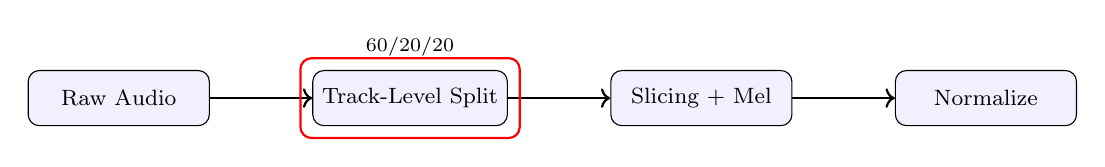
\begin{tikzpicture}[node distance=0.9cm, every node/.style={font=\footnotesize}]
      \tikzstyle{box}=[rectangle, rounded corners, draw, fill=blue!6, minimum width=2.3cm, minimum height=0.7cm]
      \node[box] (raw) {Raw Audio};
      \node[box, right=1.3cm of raw] (split) {Track-Level Split};
      \node[box, right=1.3cm of split] (slice) {Slicing + Mel};
      \node[box, right=1.3cm of slice] (std) {Normalize};
      \draw[->, thick] (raw) -- (split);
      \draw[->, thick] (split) -- (slice);
      \draw[->, thick] (slice) -- (std);
      \node[above=0.05cm of split] {\scriptsize 60/20/20};
      \draw[red, thick, rounded corners] ($(split.north west)+(-0.15,0.15)$) rectangle ($(split.south east)+(0.15,-0.15)$);
    \end{tikzpicture}
  \end{center}
\end{frame}

\begin{frame}{Methodology II: The Architectural Tournament}
  \textbf{Key Message:} Three representative CNN families compared under identical settings.\\[4pt]
  \begin{columns}[T]
    \begin{column}{0.33\textwidth}
      \textbf{1. Efficient-VGG}
      \begin{itemize}\itemsep4pt
        \item Lightweight VGG-style
        \item Strong baseline
        \item Fast inference
      \end{itemize}
    \end{column}
    \begin{column}{0.33\textwidth}
      \textbf{2. ResSE-AudioCNN}
      \begin{itemize}\itemsep4pt
        \item Residual blocks
        \item Squeeze-Excitation
        \item Deeper representation
      \end{itemize}
    \end{column}
    \begin{column}{0.33\textwidth}
      \textbf{3. U-Net Audio Classifier}
      \begin{itemize}\itemsep4pt
        \item Multi-scale encoder
        \item Skip connections
        \item Hypothesis: richer features
      \end{itemize}
    \end{column}
  \end{columns}
\end{frame}

\section{Core Results}
% ----------------------------------------------------------------------------
% GTZAN RESULTS FRAME (redesigned for more vertical breathing room)
% ----------------------------------------------------------------------------
\begin{frame}{Results on GTZAN: A Clear Performance Hierarchy}
  % Provide more space below the title so content is not squeezed to the top
  \vspace{0.12cm}
  	\textbf{Key Message:} Well-motivated complexity yields real gains.\\[6pt]
  \begin{columns}[T,totalwidth=\textwidth]
    % Text column (slightly larger item spacing for readability)
    \begin{column}{0.50\textwidth}
      \begin{itemize}\itemsep5pt
        \item Identical training protocol (SpecAugment)
        \item U-Net outperforms other CNN baselines
        \item Multi-scale feature fusion provides consistent gains
      \end{itemize}
    \end{column}
    % Chart column
    \begin{column}{0.50\textwidth}
      % Mild downward shift so chart sits visually centered relative to text
      \vspace{0.10cm}\centering
      % Baseline-relative style (Baseline = 70)
      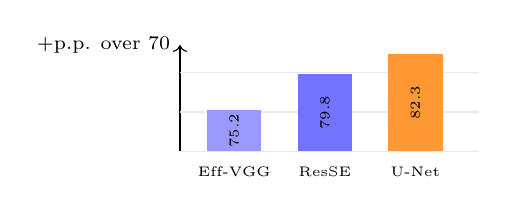
\begin{tikzpicture}[y=0.10cm, x=1.15cm]
        % Axis up to just above max diff (12.3)
        \draw[->] (0,0) -- (0,13.5) node[left]{\scriptsize +p.p. over 70};
        \draw (0,0) -- (3.3,0);
        % Grid every 5 p.p.
        \foreach \y in {0,5,10} {\draw[gray!18] (0,\y) -- (3.3,\y);}
        % Bars: raw p.p. improvements over 70
        \fill[blue!40] (0.30,0) rectangle (0.90,5.2);   % Eff-VGG 75.2
        \fill[blue!55] (1.30,0) rectangle (1.90,9.8);   % ResSE 79.8
        \fill[orange!80] (2.30,0) rectangle (2.90,12.3); % U-Net 82.3
        % Rotated numeric labels at midpoints
        \node[font=\tiny, rotate=90] at (0.60,2.6){75.2};
        \node[font=\tiny, rotate=90] at (1.60,4.9){79.8};
        \node[font=\tiny, rotate=90] at (2.60,6.15){82.3};
        % X labels
        \node[below=2pt] at (0.60,0){\tiny Eff-VGG};
        \node[below=2pt] at (1.60,0){\tiny ResSE};
        \node[below=2pt] at (2.60,0){\tiny U-Net};
      \end{tikzpicture}
    \end{column}
  \end{columns}
\end{frame}

\begin{frame}{Ablation: Why Data Augmentation Matters}
  \textbf{Key Message:} Augmentation helps only when model capacity can exploit it.\\[4pt]
  \begin{itemize}
    \item Full re-training without SpecAugment.
    \item U-Net: +0.5 p.p. gain with augmentation.
    \item Lower-capacity models: slight degradation (noise injection effect).
    \item Shows interaction between architecture depth and regularization.
  \end{itemize}
  \vspace{0.2cm}
  \begin{center}
    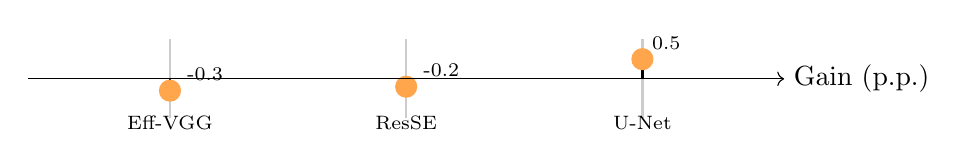
\begin{tikzpicture}[x=3cm, y=0.5cm]
      \foreach \x/\y/\n in {0/ -0.3/Eff-VGG,1/ -0.2/ResSE,2/0.5/U-Net}{
        \draw[gray!40, thick] (\x, -1) -- (\x,1);
        \draw[thick] (\x,0) -- (\x,\y);
        \fill[fill=orange!70] (\x,\y) circle (4pt);
        \node[below=0.35cm] at (\x,0) {\scriptsize \n};
        \node[above right] at (\x,\y) {\scriptsize \y};
      }
      \draw[->] (-0.6,0) -- (2.6,0) node[right]{Gain (p.p.)};
    \end{tikzpicture}
  \end{center}
\end{frame}

% PART 2 ------------------------------------------------------------------
\section{Extended Analysis}
\begin{frame}{Beyond Accuracy: Efficiency \& Complexity}
  \textbf{Key Message:} U-Net balances accuracy and efficiency better than the deeper attention model.\\[4pt]
  \begin{table}[h]
    \centering
    \begin{tabular}{lccc}
      \toprule
      Model & Test Acc. & Params (M) & Latency (ms) \\
      \midrule
      Efficient-VGG & 75.2\% & \textbf{0.03} & \textbf{14.8} \\
      ResSE-AudioCNN & 79.8\% & 1.23 & 26.8 \\
      \textbf{U-Net Audio Class.} & \textbf{82.3\%} & 1.18 & 23.1 \\
      \bottomrule
    \end{tabular}
  \end{table}
  \vspace{0.15cm}
  \begin{itemize}
    \item Efficient-VGG: minimal but sacrifices accuracy.
    \item U-Net: competitive parameter count and faster than ResSE.
    \item Practical choice for deployment among high performers.
  \end{itemize}
\end{frame}

\begin{frame}{Cross-Dataset Generalization Strategy}
     	\textbf{Key Message:} We test robustness under scale, cultural, and task shifts.\\[6pt]
  % Removed negative vspace; give columns a consistent top margin
  \begin{columns}[T,totalwidth=\textwidth]
    \begin{column}{0.33\textwidth}
      {\small \textbf{FMA Small}}\\[-3pt]
      {\tiny Open-domain scale}\\
      Larger, more diverse set.\\
      	extit{Train from scratch}
    \end{column}
    \begin{column}{0.33\textwidth}
      {\small \textbf{Indian Music}}\\[-3pt]
      {\tiny Cultural shift}\\
      Timbre / scales differ.\\
      	extit{Fine-tune upper layers}
    \end{column}
    \begin{column}{0.33\textwidth}
      {\small \textbf{Tabla Taala}}\\[-3pt]
      {\tiny Rhythmic task}\\
      Pattern emphasis.\\
      	extit{Fine-tune classifier}
    \end{column}
  \end{columns}
  \vspace{0.3cm}
  {\tiny Strategy: freeze early convolutional blocks for fine-tuning; adapt classifier head to domain/task.}
\end{frame}

\begin{frame}[t]{Results: Robustness and Adaptation}
  % Relax compression, keep frame top alignment but add space for readability
  \vspace{0.05cm}
   	\textbf{Key Message:} Strong transfer; open-domain diversity still challenging.\\[5pt]
  \begin{columns}[T,totalwidth=\textwidth]
    \begin{column}{0.46\textwidth}
      % Add minimal top padding inside column to refine vertical balance
      \vspace{0.05cm}
      \begin{itemize}\itemsep3pt
        \item Tabla Taala: \textbf{96.5\%}
        \item GTZAN: 82.3\%
        \item Indian Music: \textbf{72.2\%}
        \item FMA Small: 41.1\%
      \end{itemize}
    \end{column}
    \begin{column}{0.54\textwidth}
      % Keep chart visually high but not flush
      \vspace{-0.08cm}\centering
      % Baseline-relative style (like CV Stability). Baseline = 40.
      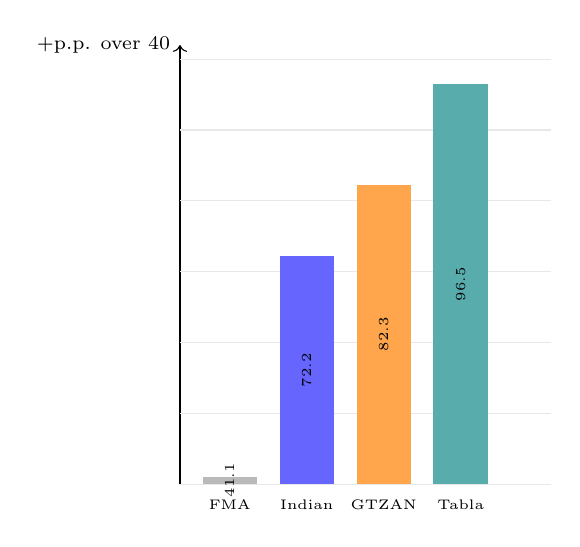
\begin{tikzpicture}[y=0.09cm, x=1.15cm]
        % Axis (0 -> ~60 p.p. over 40)
        \draw[->] (0,0) -- (0,62) node[left]{\scriptsize +p.p. over 40};
        \draw (0,0) -- (4.1,0);
        % Grid every 10 p.p.
        \foreach \y in {0,10,20,30,40,50,60} {\draw[gray!18] (0,\y) -- (4.1,\y);}
        % Heights over 40: FMA 1.1, Indian 32.2, GTZAN 42.3, Tabla 56.5
        \fill[gray!55]   (0.25,0) rectangle (0.85,1.1);  % FMA
        \fill[blue!60]   (1.10,0) rectangle (1.70,32.2); % Indian
        \fill[orange!70] (1.95,0) rectangle (2.55,42.3); % GTZAN
        \fill[teal!65]   (2.80,0) rectangle (3.40,56.5); % Tabla
        % Rotated numeric labels mid-bar
        \node[font=\tiny, rotate=90] at (0.55,0.55){41.1};
        \node[font=\tiny, rotate=90] at (1.40,16.1){72.2};
        \node[font=\tiny, rotate=90] at (2.25,21.15){82.3};
        \node[font=\tiny, rotate=90] at (3.10,28.25){96.5};
        % X labels
        \node[below=2pt] at (0.55,0){\tiny FMA};
        \node[below=2pt] at (1.40,0){\tiny Indian};
        \node[below=2pt] at (2.25,0){\tiny GTZAN};
        \node[below=2pt] at (3.10,0){\tiny Tabla};
      \end{tikzpicture}
    \end{column}
  \end{columns}
\end{frame}

\begin{frame}{Cross-Validation Stability}
  	\textbf{Key Message:} Consistent fold performance – narrow variance band.\\[4pt]
  \begin{itemize}\itemsep3pt
    \item U-Net 5-fold CV on GTZAN (track-level splits)
    \item Mean: \textbf{90.44\%} \quad Std: \textbf{0.68 p.p.}
    \item Max/Min: 91.44\% / 89.44\% \ (range 2.0 p.p.)
    \item Supports reliability of reported single-split test score.
  \end{itemize}
  % Slight negative space so the per-fold bar plot sits higher
  \vspace{-0.05cm}
  \centering
  % Compact per-fold bars (mapping 89% baseline to 0). Raised with yshift.
  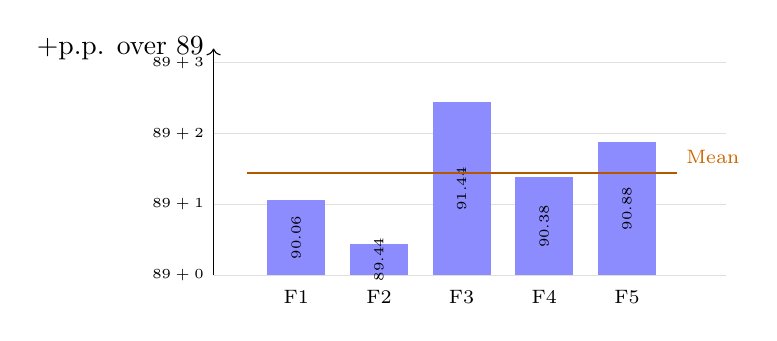
\begin{tikzpicture}[y=0.9cm, x=1.05cm, yshift=20pt]
    % Axes
    \draw[->] (0,0) -- (0,3.2) node[left]{+p.p. over 89};
    \draw (0,0) -- (6.2,0);
    % Grid and y tick labels
    \foreach \y in {0,1,2,3} {\draw[gray!25] (0,\y) -- (6.2,\y); \node[left, font=\tiny] at (0,\y){$89+\y$};}
    % Bars (heights = value - 89)
    \fill[blue!45] (0.65,0) rectangle (1.35,1.06); % 90.06
    \fill[blue!45] (1.65,0) rectangle (2.35,0.44); % 89.44
    \fill[blue!45] (2.65,0) rectangle (3.35,2.44); % 91.44
    \fill[blue!45] (3.65,0) rectangle (4.35,1.38); % 90.38
    \fill[blue!45] (4.65,0) rectangle (5.35,1.88); % 90.88
    % Numeric labels
    \node[font=\tiny, rotate=90] at (1.00,0.53){90.06};
    \node[font=\tiny, rotate=90] at (2.00,0.22){89.44};
    \node[font=\tiny, rotate=90] at (3.00,1.22){91.44};
    \node[font=\tiny, rotate=90] at (4.00,0.69){90.38};
    \node[font=\tiny, rotate=90] at (5.00,0.94){90.88};
    % X labels
    \foreach \x/\l in {1/F1,2/F2,3/F3,4/F4,5/F5} {\node[below=2pt] at (\x,0){\scriptsize \l};}
    % Mean line only (removed std band rectangle)
    \def\meanShift{1.44}
    \draw[thick, orange!70!black] (0.4,\meanShift) -- (5.6,\meanShift);
    \node[font=\scriptsize, orange!80!black, above right] at (5.6,\meanShift){Mean};
  \end{tikzpicture}
\end{frame}

\section{Conclusion}
\begin{frame}{Conclusion \& Key Takeaways}
  \textbf{Key Message:} We provide a rigorous benchmark and validate a strong architecture.\\[4pt]
  \begin{itemize}
    \item Leak-free methodology is \textbf{essential} for trustworthy MGC results.
    \item U-Net encoder delivers ~90.4\% (CV) / 82.3\% (test) on GTZAN.
    \item Transfer learning unlocks high performance in new domains (Tabla 96.5\%).
    \item Provides a transparent, reproducible baseline for future work.
  \end{itemize}
\end{frame}

\begin{frame}[plain]
  \centering
  {\Huge \textbf{Thank You}}\par\vspace{0.5cm}
  {\Large Questions?}\\[0.6cm]
  {\normalsize Alessandro Potenza \& Camilla Sed}\\[0.2cm]
  {\footnotesize GitHub: \url{https://github.com/alepot55/MGC-GTZAN}}
\end{frame}

% Optional references frame (commented)
% \begin{frame}{References}
%   \bibliography{../reports/final_paper/bibliography.bib}
%   \bibliographystyle{apalike}
% \end{frame}

\end{document}